\chapter{Monitoraggio e Kubernetes} \label{chap:monitorin-kubernetes}

\section{Monitoring}

Per comprendere al meglio il funzionamento di Prometheus, è necessario prima comprendere cosa sia il concetto di monitoraggio stesso e in che modo può essere utilizzato.

\subsection{Cosa è?}
Il monitoring è un processo che si basa principalmente \textbf{sull'osservazione costante dello stato di salute un sistema}, con l'obiettivo di individuare eventuali anomalie prima che queste possano causare disservizi agli utenti. \\
In particolare, nel modello DevOps, il monitoring funge da congiunzione tra le operazioni di sviluppo e quelle operazionali, perché la raccolta di dati in tempo reale sulle prestazioni e la salute del sistema permette di poter pianificare in maniera più accurata le successive iterazioni, favorendo un’evoluzione rapida e continua, permettendo di rispondere efficacemente alle nuove esigenze che nascono durante la vita di un software.

\subsection{Logging vs Monitoring vs Alerting} 
Spesso logging e monitoring vengono considerati come attività distinte o addirittura in competizione, ma in realtà sono \textbf{complementari}. Mentre il logging si focalizza sulla \textbf{registrazione degli eventi} che si verificano all'interno del sistema, il monitoring si occupa di \textbf{monitorare lo stato attuale} del sistema. La combinazione di entrambe le tecniche permette di affrontare in maniera più efficiente il \textit{troubleshooting}: i log forniscono dettagli sugli eventi anomali, mentre le metriche del monitoraggio mostrano lo stato del sistema nel momento in cui tali eventi si sono verificati. Questo approccio integrato consente di analizzare i problemi in modo più approfondito e accurato. \\
L’alerting, invece, è strettamente legato al monitoraggio e si riferisce all’insieme delle operazioni finalizzate a \textbf{notificare in modo tempestivo il verificarsi di una condizione critica}. Esempi includono l’eccessivo utilizzo delle risorse in un cluster, o un incremento anomalo nei tempi di risposta a richieste HTTP per un periodo prolungato. \\
Sebbene concettualmente semplice, l’alerting è di fondamentale importanza poiché permette di evitare il degrado del sistema e di avviare prontamente operazioni di troubleshooting. Inoltre, l’alerting comporta una serie di \textbf{considerazioni tecniche}, come il filtraggio degli alert, la scelta della loro severità, la selezione del canale di comunicazione più adatto e altri fattori che incidono direttamente sull’efficacia delle operazioni di monitoraggio.



\section{Kubernetes}
La campagna di fault injection nasce proprio con l'idea di studiare in maniera sistematica gli errori che possono scatenarsi in un cluster \textbf{Kubernetes} \cite{Kubernetes}, quindi per comprendere cosa viene effettivamente monitorato in un cluster e in che modo avviene tale processo con Prometheus, anche in questo caso è necessario prima comprendere come funziona Kubernetes stesso.

\subsection{Cosa è?}

Kubernetes è un \textbf{orchestratore di container}, ovvero un framework che si occupa sia di automatizzare tutte le operazioni per la gestione di quest'ultimi sia di garantire determinate specifiche (che possono essere di diverse tipologie, ad esempio sotto forma di risorse da utilizzare, di scalabilità e così via...) occupandosi quindi di gestire l'intero ciclo di vita di un container.
\\
Inizialmente sviluppato da Google, poi donato alla Cloud Native Computing Foundation \cite{CNCF} rendendolo così un software open source, ad oggi è diventato un de facto standard per questa tipologia di strumenti.
\\
Ma prima di approfondirlo è doveroso introdurre i container.

\subsection{Container}
\begin{figure}[ht]
    \centering
    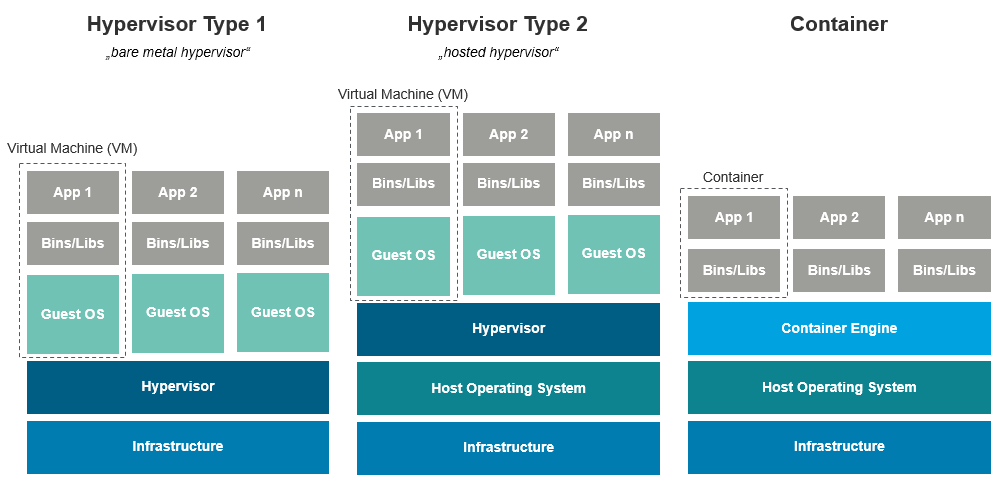
\includegraphics[width=0.95\linewidth]{UNINA_BSc_Final_Report//img//explanation/VM vs Container.png}
    \caption{confronto virtualizzazione e containerizzazione \cite{Vm-vs-Container}}
    \label{fig:Container}
\end{figure}
Un container non è altro che un pacchetto che racchiude del codice software e tutti i componenti necessari per eseguirlo correttamente, come librerie e altre dipendenze, tutte incorporate in una singola struttura. \\
La containerizzazione di un applicazione porta numerosi vantaggi, innanzitutto grazie all'isolamento dell'applicazione quest'ultima potrà essere eseguita in maniera \textbf{indipendente dall'ambiente} in cui si trova, ad esempio a prescindere dal sistema operativo dell'host, ma il principale vantaggio è dato dalla \textbf{portabilità} e \textbf{leggerezza} di questi ultimi, infatti a differenza di una macchina virtuale che può essere vista come un sistema a sé stante, un container invece può essere visto come un'estensione di un classico processo di un sistema operativo e \textbf{non necessita della virtualizzazione delle risorse}, ma lavora direttamente condividendo il Kernel dell'host [fig. \ref{fig:Container}]. \\
Sfruttano tecnologie come i \textit{namespace}, che permettono di isolare un insieme di risorse, e i \textit{cgroups}, che permettono invece di definire e limitare l'utilizzo delle risorse da parte di un gruppo di processi ad esempio di uno stesso namespace. Questo permette di \textbf{ridurre drasticamente l'utilizzo delle risorse} come lo spazio sul disco e in memoria, i tempi di avvio, etc... anche in termini di ordini di grandezza, semplificando la scalabilità di un applicazione.
\\
I container a loro volta non sono altro che delle \textbf{istanze} di quelle che vengono chiamate \textbf{immagini},
definibili come l'analogo delle classi nella programmazione a oggetti, ma queste vengono a loro volta create effettuando un processo di \textbf{build} tramite appositi file di configurazione ed inoltre sarà anche necessario rilasciare e scalare opportunamente tali container. Questo insieme di operazioni dovrebbe poi essere ripetuto per ogni singolo container (che possono facilmente arrivare ad esserne centinaia), ed è per questo scopo che sono nati strumenti come Kubernetes che si occupano di \textbf{automatizzare} tutte queste operazioni.

\subsection{Architettura}
\begin{figure}[ht]
    \centering
    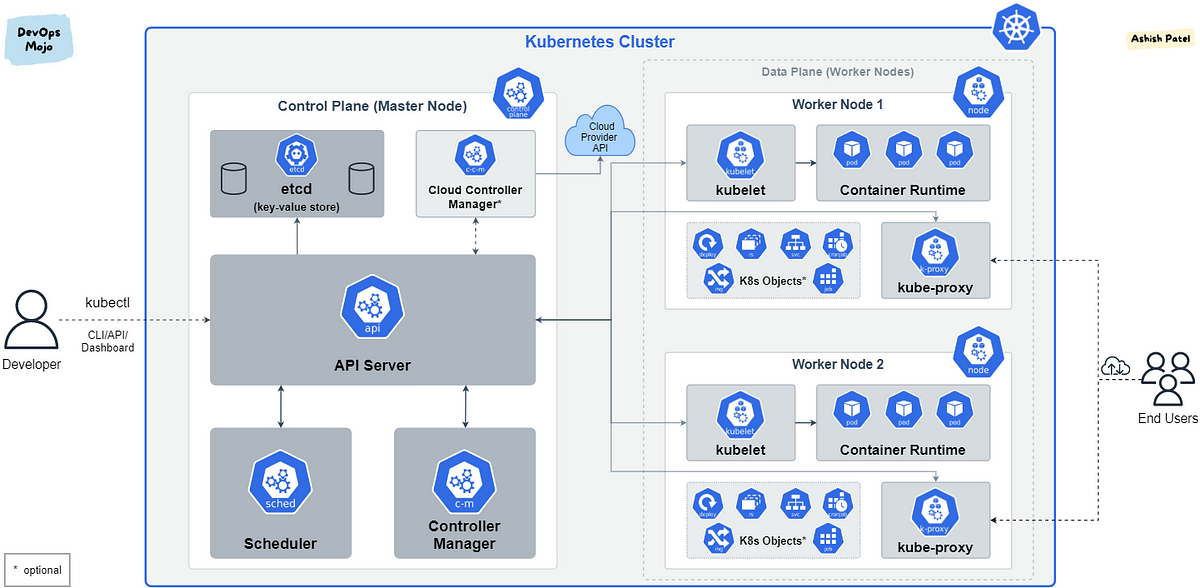
\includegraphics[width=1\linewidth]{UNINA_BSc_Final_Report//img//explanation/kubernetes-cluster-architecture-DevOps.png}
    \caption{architettura di un cluster Kubernetes \cite{k8s-architecture}}
    \label{fig:k8s-architecture}
\end{figure}
Come si può intuire Kubernetes è uno strumento complesso, ed è per questo che per semplificarne lo sviluppo e la comprensibilità è stato suddiviso in diverse componenti coese, raggruppate in quello che viene definito \textbf{cluster} [fig. \ref{fig:k8s-architecture}]: un insieme di macchine comunicanti tra di loro sulla quale vengono eseguite sia tali componenti, sia i container della nostra applicazione.
\\
Un cluster generalmente utilizza uno schema master / worker, ovvero alcune macchine fungeranno da \textbf{Control Plane} (dette \textbf{nodi master}) che si occuperanno di gestire le restanti macchine (dette \textbf{nodi} / \textbf{nodi worker}) sulla quale verranno eseguiti i \textbf{pod} (gruppi di container) ed altre tipologie di \textbf{oggetti} di Kubernetes.
\\
Sia i nodi master che i worker, oltre ad eseguire gli oggetti specifici del sistema che si vuole creare, devono necessariamente eseguire alcune componenti che garantiscono il corretto funzionamento del cluster, ovvero:
\begin{itemize}
    \item \textbf{Control Plane}
        \begin{itemize} 
            \item \textbf{kube-apiserver} \\
            espone le \textbf{API} di Kubernetes e processa le richieste \textbf{REST} o del tool di command line \textbf{kubectl}.
            \item \textbf{etcd} \\
            database persistente, stateful e key-value, contenente tutte le informazioni riguardanti lo stato del cluster.
            \item \textbf{kube-scheduler} \\
            assegna i nuovi pod ai nodi worker in base a diversi criteri.
            \item \textbf{kube-controller-manager} \\
            controlla lo stato desiderato degli oggetti nel cluster e lo confronta con lo stato attuale tramite l'Apiserver, eventualmente applica degli step correttivi per riconciliarli.
        \end{itemize}
    \item \textbf{Nodi}
        \begin{itemize} 
            \item \textbf{kubelet} \\
            intermediario tra l'Apiserver e il nodo, seguendo le istruzioni del nodo master avvia e controlla i pod nei nodi worker.
            \item \textbf{container runtime} \\
            motore per scaricare, eseguire e gestire i container nei pod.
            \item \textbf{kube-proxy} \\
            network proxy che si occupa della gestione delle comunicazioni con i pod internamente ed esternamente.
        \end{itemize}
\end{itemize}
Tutte queste componenti sono \textbf{stateless} e \textbf{comunicano indirettamente} tra di loro utilizzando l'Etcd, ma solo l'Apiserver può accederci e quindi la comunicazione avviene unicamente tramite l'invocazione delle apposite API. \\
Questo pattern rende l'Etcd un \textbf{componente critico}, ed è proprio su tale criticità che è stata basata la campagna di fault/error injection, dove le iniezioni sono state effettuate proprio nella comunicazione tra Apiserver e Etcd.

%*******************************************************************************************************%

\section{Perché Prometheus?}
\textbf{Prometheus} \cite{Prometheus} è un framework di \textbf{monitoraggio} e \textbf{alerting} ormai maturo, che mette a disposizione numerose funzionalità extra come l' immagazzinamento dei dati in maniera persistente, un apposito linguaggio di interrogazione sui dati, etc... che verranno approfondite nel prossimo capitolo.
\\
Ma la vera differenza con i suoi competitor è del far parte della CNCF \cite{CNCF}, perché essendo un progetto open source la sua grande diffusione permette di creare una vasta \textbf{community} attiva, di fondamentale importanza dato che chiunque può realizzare una propria fork del progetto, chiunque può creare dei nuovi moduli per monitorare sistemi e strumenti non ufficialmente supportati (basta dare una rapida occhiata alle loro liste \cite{Prometheus-clients-exporters-list} per vedere come la maggioranza siano sviluppate dalla community), gli aggiornamenti sono continui, le vulnerabilità vengono rilevate e corrette rapidamente e soprattutto la \textbf{documentazione} che si può trovare online è immensamente maggiore rispetto a molte sue alternative. \\
In realtà infatti potremmo dire che Prometheus non abbia dei veri e propri competitor considerata la sua community, ma bensì che esistano delle soluzioni alternative che si focalizzano su specifici obbiettivi, ad esempio per citarne alcune:
\begin{itemize}
    \item \textbf{InfluxDB} \cite{InfluxDB}: particolarmente efficiente in termini di risorse, ha un linguaggio di interrogazione più semplice da utilizzare e più rapido, ma ha un ecosistema decisamente più acerbo e risulta essere più complesso da configurare.
    \item \textbf{Graphite} \cite{Graphite}: punta tutto sulla semplicità di configurazione e d'uso, ma allo stesso tempo ha meno funzionalità di interrogazione e non è molto adatto per ambienti di monitoraggio complessi.
    \item \textbf{VictoriaMetrics} \cite{VictoriaMetrics}: probabilmente l'alternativa che più si avvicina a Prometheus, infatti può essere vista come una sua variante ma con l'obiettivo di avere un footprint minore ed offre anche un linguaggio di interrogazione più avanzato, ma al costo di avere meno funzionalità ed un ecosistema decisamente meno maturo, quindi con documentazione online e supporto della community inferiore.
\end{itemize}
Quindi anche se esistono numerose altre alternative, analogamente a quanto successo con Kubernetes, anche Prometheus è diventato un de facto standard nel suo ambiente.